\documentclass[11pt]{article}
\usepackage[T1]{fontenc}
\usepackage{amsmath,amssymb,amsthm,mathtools}
\usepackage[margin=0.88in]{geometry}
\usepackage{graphicx}
\usepackage{microtype}
\usepackage{xcolor}
\usepackage[colorlinks=true,linkcolor=blue!55!black,urlcolor=blue!55!black,citecolor=blue!55!black]{hyperref}

\newtheorem{theorem}{Theorem}
\newtheorem{proposition}[theorem]{Proposition}
\newtheorem{remark}[theorem]{Remark}
\newcommand{\C}{\mathbb C}
\newcommand{\R}{\mathbb R}
\newcommand{\Id}{\mathsf I}
\newcommand{\Dzero}{\mathsf D_0}
\newcommand{\op}{\operatorname}

\title{Clifford scalar potentials and Dirac confinement\\in every dimension}
\author{Automated Math Discovery Run \texttt{fa\_banach\_001}, lane 8}
\date{11 August 2026}

\begin{document}
\maketitle

\begin{center}
\fcolorbox{black}{red!5}{\parbox{0.91\linewidth}{
\textbf{Result.} The Clifford-algebra problem in Comment 5 of
Nenciu--Nenciu--Obermeyer is solved for the minimal Hamiltonian spinor in every
dimension.  The scalar-potential space has real dimension one for even spatial
dimension and two for odd spatial dimension.  The source confinement theory
extends to this full class, and the fixed-mass boundary threshold
$|\lambda|=1/2$ is sharp in every dimension.}}
\end{center}

\section{Source question}

Nenciu, Nenciu, and Obermeyer \cite{NNO} define a Hermitian matrix potential
$V$ to be \emph{scalar} when it anticommutes with every principal Dirac matrix.
Their Comment 5 asks for free Dirac matrices in all dimensions, the complete
class $\mathcal S_s$ of such potentials, and the analogue of their
Lorentz-scalar theory.  They separately ask whether the optimal boundary
growth rate is dimension-independent.  The question is on PDF pages 34--35.

\begin{center}
  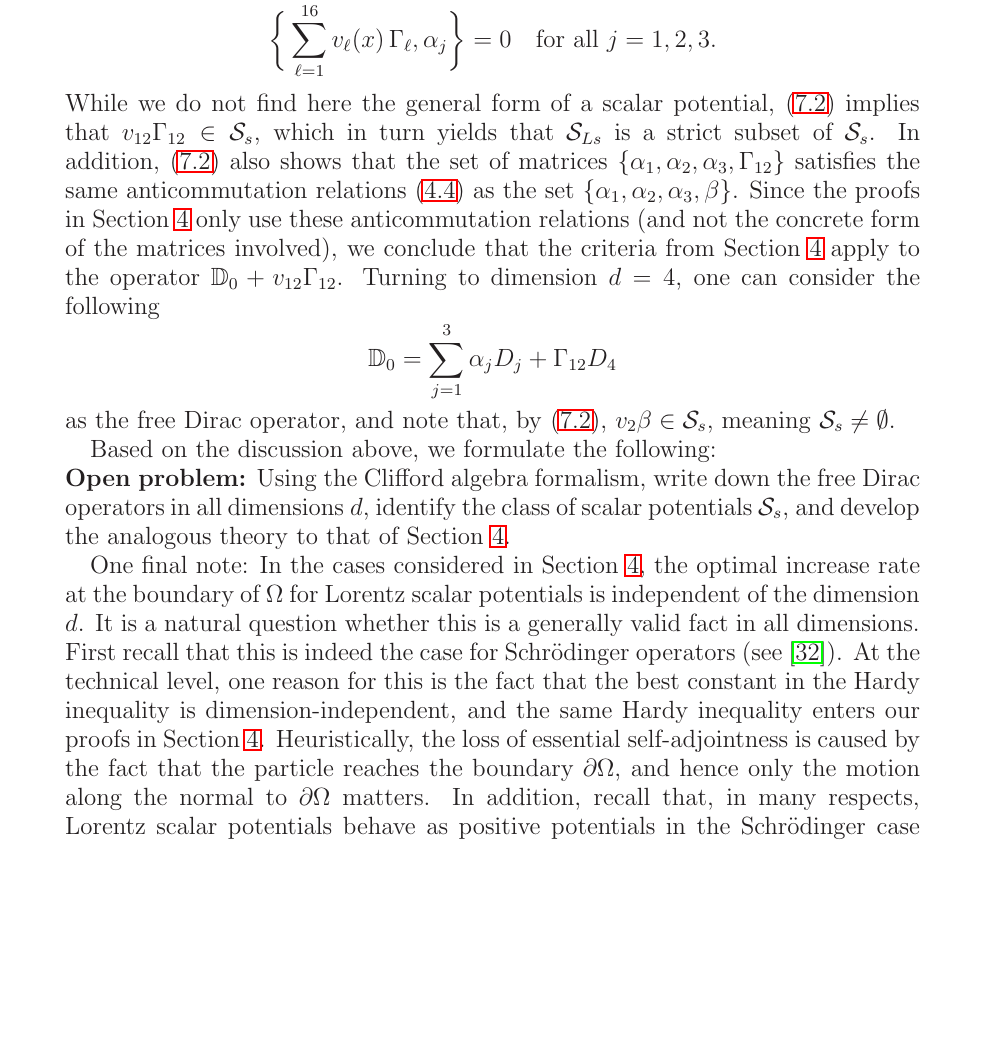
\includegraphics[width=0.97\linewidth]{figures/open_problem_crop_page34.png}
  \par\smallskip\small Figure 1. The algebraic problem and the
  dimension-independence question, arXiv:2010.09816, PDF page 34.
\end{center}

\begin{center}
  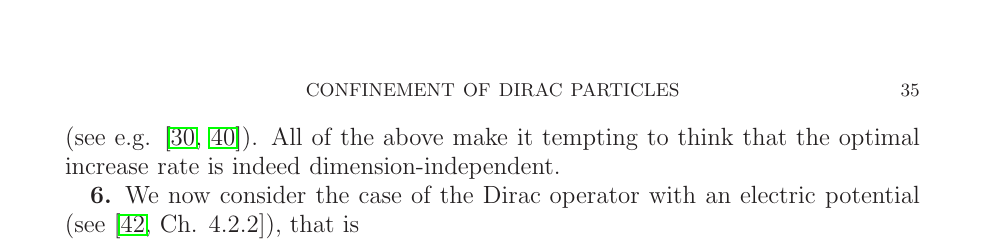
\includegraphics[width=0.97\linewidth]{figures/open_problem_crop_page35.png}
  \par\smallskip\small Figure 2. The final two lines of the
  dimension-independence question, PDF page 35.
\end{center}

\section{Explicit all-dimensional model}

Let $d\geq1$ and $N_d=2^{\lfloor(d+1)/2\rfloor}$.  Write $X,Y,Z$ for the
Pauli matrices.  The standard Jordan--Wigner matrices give an explicit
irreducible complex representation of $\mathrm{Cl}_{d+1}$: if
$m=\lfloor(d+1)/2\rfloor$, put
\begin{align*}
 \gamma_{2j-1}&=Z^{\otimes(j-1)}\otimes X\otimes
                  \Id^{\otimes(m-j)},\\
 \gamma_{2j}&=Z^{\otimes(j-1)}\otimes Y\otimes
                  \Id^{\otimes(m-j)},\qquad 1\leq j\leq m,
\end{align*}
retaining only indices at most $d+1$; when $d+1=2m+1$, append
$\gamma_{2m+1}=Z^{\otimes m}$.  Thus
\[
 \gamma_j^*=\gamma_j,
 \qquad \gamma_j\gamma_k+\gamma_k\gamma_j=2\delta_{jk}\Id.
\]
Set $\alpha_j=\gamma_j$ for $1\leq j\leq d$, $\beta=\gamma_{d+1}$, and
\[
 \Dzero=-i\sum_{j=1}^d\alpha_j\partial_j,
 \qquad
 \Gamma_d=i^{d(d-1)/2}\alpha_1\cdots\alpha_d.
\]
The phase makes $\Gamma_d$ a Hermitian involution.  It anticommutes with each
$\alpha_j$ for even $d$ and commutes with each $\alpha_j$ for odd $d$.

\section{Proof intuition}

Multiplication by the already available mass matrix $\beta$ turns an
anticommuting matrix into a commuting one.  The problem is therefore exactly a
commutant calculation for the restriction from $\mathrm{Cl}_{d+1}$ to
$\mathrm{Cl}_d$.  That restriction is irreducible in even $d$, but splits into
the two inequivalent irreducibles in odd $d$; the volume element $\Gamma_d$
distinguishes the two summands.  This parity fact produces either one or two
real mass directions.

Once these directions are known, their Clifford relations collapse $V^2$ to
the Euclidean squared length of the coefficient vector.  The source paper's
coercivity matrix can then be bounded by a scalar expression.  For a fixed
mass direction, the critical proof is literally dimension-free: the matrices
$iM\alpha_j$ again form a Clifford family and
$\|\Dzero\phi\|_2^2=\|\nabla\phi\|_2^2$.  On the unit ball the normal equation
has exponents $\pm\lambda$, so square integrability changes precisely at
$|\lambda|=1/2$.

\section{Classification theorem}

For a point $x$, let
\[
 \mathcal S_s(x)=\{V=V^*\in M_{N_d}(\C):
       \alpha_jV+V\alpha_j=0\text{ for }j=1,\dots,d\}.
\]

\begin{theorem}[Complete scalar-potential classification]\label{thm:class}
For the minimal Hamiltonian spinor model above,
\[
 \mathcal S_s(x)=
 \begin{cases}
   \{v(x)\beta:v(x)\in\R\},& d\text{ even},\\[2mm]
   \{v_1(x)\beta+v_2(x)\widetilde\beta:
             v_1(x),v_2(x)\in\R\},&d\text{ odd},
 \end{cases}
 \qquad \widetilde\beta=i\beta\Gamma_d.
\]
For odd $d$, $\beta$ and $\widetilde\beta$ are anticommuting Hermitian
involutions.  Consequently
\[
 (v_1\beta+v_2\widetilde\beta)^2=(v_1^2+v_2^2)\Id.
\]
In the standard $d=3$ matrices of \cite{NNO},
$\widetilde\beta=-\Gamma_{12}$, up to the harmless choice of orientation.
Hence the two matrices displayed in Comment 5 span the entire class.
\end{theorem}

\begin{proof}
Let $V$ anticommute with all $\alpha_j$ and put $C=\beta V$.  Twice using
anticommutation gives $\alpha_jC=C\alpha_j$, so $C$ belongs to the commutant of
the restricted $\mathrm{Cl}_d$ representation.

If $d$ is even, complex $\mathrm{Cl}_d$ is a full matrix algebra and its action
on $\C^{N_d}$ is irreducible.  Schur's lemma gives $C=c\Id$, hence
$V=c\beta$; Hermiticity forces $c\in\R$.

If $d$ is odd, the restriction is the multiplicity-one sum of the two
inequivalent irreducible $\mathrm{Cl}_d$ modules.  The two eigenspaces of the
central volume element $\Gamma_d$ are precisely those summands.  Therefore its
commutant is $\op{span}_{\C}\{\Id,\Gamma_d\}$.  Thus
$V=a\beta+c\beta\Gamma_d$.  Since $\beta\Gamma_d=-\Gamma_d\beta$ is
skew-Hermitian, $V=V^*$ holds exactly when $a\in\R$ and $c=ib$ with
$b\in\R$.  This proves the displayed classification.

For odd $d$, $\beta$ anticommutes with $\Gamma_d$.  Direct multiplication now
shows that $i\beta\Gamma_d$ is Hermitian, squares to $\Id$, and anticommutes
with $\beta$ and every $\alpha_j$.  The square formula follows.  Substitution
of the standard $d=3$ matrices gives $i\beta\Gamma_3=-\Gamma_{12}$.
\end{proof}

\section{The full mass-vector confinement criterion}

Let $q_d=1$ in even dimensions and $q_d=2$ in odd dimensions.  Denote the
mass frame by $B_1=\beta$, and, in odd dimensions, $B_2=\widetilde\beta$.
For $u=(u_1,\dots,u_{q_d})\in C^1(\Omega;\R^{q_d})$, set
$V_u=\sum_a u_aB_a$.  Let $\widehat\delta$ be the regularized distance used in
\cite[Theorem 2.2]{NNO} and put $h=\log\widehat\delta$.

\begin{theorem}[All-dimensional scalar criterion]\label{thm:coercive}
The source coercivity matrix \cite[Theorem 2.5]{NNO} specializes exactly to
\begin{equation}\label{eq:Q}
 Q_{u,h}=|u|^2\Id-i\sum_{j=1}^d\alpha_j\partial_jV_u
       -2i\alpha(\nabla h)V_u-|\nabla h|^2\Id.
\end{equation}
If $Q_{u,h}\geq c\Id$ near $\partial\Omega$ for some $c>0$, then
$\Dzero+V_u$ is essentially self-adjoint on
$C_c^1(\Omega;\C^{N_d})$.  In particular, it is sufficient that
\begin{equation}\label{eq:scalarbound}
 |u|^2-\sqrt d\,|\nabla u|_{\mathrm F}
 -2|u|\,|\nabla h|-|\nabla h|^2\geq c
\end{equation}
near the boundary.

Consequently, let $a>1$.  If for some $\varepsilon>0$ and positive $c,C$,
\begin{equation}\label{eq:supercritical}
 c\delta^{-a}\leq |u|\leq C\delta^{-(2a-1-\varepsilon)},
 \qquad |\nabla u|_{\mathrm F}\leq C\delta^{-(2a-\varepsilon)}
\end{equation}
when $\delta=\op{dist}(x,\partial\Omega)$ is small, then
$\Dzero+V_u$ is essentially self-adjoint.
\end{theorem}

\begin{proof}
Theorem~\ref{thm:class} gives $V_u^2=|u|^2\Id$.  Since every
$\partial_jV_u$ anticommutes with $\alpha_j$,
\[
 -\frac i2\sum_j(\alpha_j\partial_jV_u-\partial_jV_u\alpha_j)
 =-i\sum_j\alpha_j\partial_jV_u.
\]
Likewise $-i[\alpha(\nabla h),V_u]=-2i\alpha(\nabla h)V_u$ and
$\alpha(\nabla h)^2=|\nabla h|^2\Id$.  This is \eqref{eq:Q}, and the first
claim is exactly \cite[Theorem 2.5]{NNO} with the constant Dirac velocity
matrix.

Moreover $\|\partial_jV_u\|=|\partial_ju|$ and
$\|\alpha(\nabla h)V_u\|=|\nabla h|\,|u|$.  The triangle and Cauchy--Schwarz
inequalities give \eqref{eq:scalarbound}.  Finally
$|\nabla h|=O(\delta^{-1})$.  Under \eqref{eq:supercritical}, the negative
terms in \eqref{eq:scalarbound} are respectively
$O(\delta^{-2a+\varepsilon})$,
$O(\delta^{-2a+\varepsilon})$, and $O(\delta^{-2})$, whereas
$|u|^2\geq c^2\delta^{-2a}$.  Since $a>1$, the positive term dominates.
\end{proof}

\section{Critical rate and its sharpness}

\begin{theorem}[Dimension-free sharp threshold]\label{thm:critical}
Let $\Omega\subset\R^d$ be bounded with $C^2$ codimension-one boundary, let
$M$ be any constant Hermitian involution anticommuting with every $\alpha_j$,
and suppose, near the boundary,
\[
 V(x)=\lambda\frac{\ell(x)}{\delta(x)}M,
 \qquad |\ell|\geq1,
 \qquad |\nabla(\ell/\delta)|\leq C|\ell|/\delta^2.
\]
Put
$\mu=\limsup_{\delta(x)\to0}\delta(x)|\nabla\ell(x)|/|\ell(x)|$.
Then $\Dzero+V$ is essentially self-adjoint whenever
$|\lambda|>(1+\mu)/2$.  Its closed domain is independent of $|\lambda|$ in
this range.  If $\Omega$ is convex and $\ell=1$ near the boundary, the endpoint
$|\lambda|=1/2$ is included.

For the unit ball $B^d$, the operator
\[
 \Dzero+\frac{\lambda}{1-|x|}M
 \quad\text{on }C_c^1(B^d;\C^{N_d})
\]
is essentially self-adjoint if and only if $|\lambda|\geq1/2$.
Thus both the critical growth exponent one and the coefficient $1/2$ are
dimension-independent and optimal.
\end{theorem}

\begin{proof}
The proof of \cite[Theorem 4.3]{NNO} is algebraic except for the scalar Hardy
inequality.  Replacing its three-dimensional $\beta$ by $M$, the matrices
$iM\alpha_j$ are Hermitian and satisfy the same Clifford relations as the
$\alpha_j$.  Hence the paper's key matrix $B(x)$ still obeys
\[
 B(x)^2=\left| -\nabla\delta(x)
       +\delta(x)\frac{\nabla\ell(x)}{\ell(x)}\right|^2\Id.
\]
Also, on compactly supported spinors in every dimension,
\[
 \|\Dzero\phi\|_2^2=\langle\phi,-\Delta\phi\rangle
 =\|\nabla\phi\|_2^2,
\]
so the same weak Hardy bound with coefficient $1/4$ enters.  Every subsequent
estimate in the proof of \cite[Theorem 4.3]{NNO} is scalar.  It therefore gives
$|\lambda|>(1+\mu)/2$, the domain statement, and, using the convex-domain Hardy
remainder, the endpoint $|\lambda|=1/2$ without any dimension restriction.

It remains to prove sharpness.  On $B^d$, the standard spinor spherical
decomposition \cite[Chapter 4]{Thaller} (the same partial-wave mechanism cited
in \cite[Section 5]{NNO})
unitarily decomposes the operator into radial first-order systems.  After the
usual multiplication by $r^{(d-1)/2}$, every channel has, near $r=1$, the form
\[
 -iJ\frac d{dr}+\frac{\lambda}{1-r}K+R_\kappa(r),
\]
where $J,K$ are anticommuting Hermitian matrices and $R_\kappa$ is bounded near
$r=1$; the angular eigenvalue contributes only a multiple of $1/r$.
Writing $t=1-r$, the residue matrix is unitarily equivalent to
$i\lambda\alpha_rM$ and has eigenvalues $\pm\lambda$.  Standard
regular-singular ODE theory therefore gives a fundamental pair with sizes
$t^{|\lambda|}$ and $t^{-|\lambda|}$, up to bounded invertible factors (and
harmless logarithms in resonant cases).  Both are in $L^2(0,\varepsilon;dt)$
exactly when $|\lambda|<1/2$.  The outer endpoint is then limit-circle, so a
radial channel, and hence the minimal ball operator, is not essentially
self-adjoint.  The already proved convex-domain result supplies essential
self-adjointness for $|\lambda|\geq1/2$.
\end{proof}

\section{Odd-dimensional mass rotation}

\begin{proposition}[Exact gauge formula]\label{prop:gauge}
Let $d$ be odd, $\rho,\theta\in C^1(\Omega;\R)$, and
\[
 V=\rho(\cos\theta\,\beta+\sin\theta\,\widetilde\beta),
 \qquad U_\theta=e^{-i\theta\Gamma_d/2}.
\]
Then $U_\theta$ commutes with every $\alpha_j$,
$U_\theta\beta U_\theta^*=\cos\theta\,\beta+\sin\theta\,\widetilde\beta$, and
\begin{equation}\label{eq:gauge}
 U_\theta^*(\Dzero+V)U_\theta
 =\Dzero+\rho\beta-\frac12\alpha(\nabla\theta)\Gamma_d.
\end{equation}
In particular, bounded $\nabla\theta$ does not change essential
self-adjointness; more singular rotations are covered directly by
Theorem~\ref{thm:coercive} when its scalar bound holds.
\end{proposition}

\begin{proof}
For odd $d$, $\Gamma_d$ commutes with the kinetic matrices and anticommutes
with $\beta$.  Expanding the exponential on the two eigenspaces of $\Gamma_d$
gives the rotation identity.  The product rule gives
$U_\theta^*\partial_jU_\theta=-i(\partial_j\theta)\Gamma_d/2$, which yields
\eqref{eq:gauge}.  If $\nabla\theta$ is bounded, the last term is a bounded
Hermitian perturbation.
\end{proof}

\section{Verification, novelty, and limitations}

The script \texttt{code/verify\_clifford\_classification.py} constructs the
Jordan--Wigner matrices, solves the complex matrix anticommutation system for
$d=1,\dots,8$, and obtains dimensions $2,1,2,1,2,1,2,1$, exactly as predicted.
It checks all mass-frame relations, random mass-vector square identities
(worst residual $2.802\times10^{-17}$), and the normal residue eigenvalues for
five values of $\lambda$ in every tested dimension.  The full command and
output are in \texttt{code/verifier\_report.txt}.  These checks are not used as
proof.

A bounded official-arXiv search through 11 August 2026 used arXiv id
2010.09816, the exact phrases ``scalar potentials'' and ``Clifford algebra'',
and combinations of ``Dirac confinement'', ``all dimensions'', and
``essential self-adjointness''.  It found the source paper but no later exact
answer to Comment 5 or the dimension-free threshold question.  Novelty still
requires expert review.

The theorem concerns the natural minimal Hamiltonian spinor representation
specified above.  Direct sums with extra multiplicity have larger
matrix-valued commutants and require the corresponding multiplicity-space
version of the classification.  The packet does not solve the separate
electric-potential or generic higher-dimensional magnetic-confinement problems
in Comments 6 and 8.  Human review should focus on the radial-channel
limit-point argument and on matching the source's domain conventions at the
critical endpoint.

\begin{thebibliography}{9}
\bibitem{NNO}
G.~Nenciu, I.~Nenciu, and R.~Obermeyer,
\emph{Essential self-adjointness of symmetric first-order differential systems
and confinement of Dirac particles on bounded domains in $\R^d$},
arXiv:2010.09816v2, 2021.

\bibitem{Thaller}
B.~Thaller, \emph{The Dirac Equation}, Texts and Monographs in Physics,
Springer, 1992.  See Chapter 4 for partial-wave decompositions.
\end{thebibliography}

\end{document}
